\documentclass[11pt,a4paper]{article}



% abstract
\def\abstract{%
    \quotation\small }
\def\endabstract{\vspace{1.6em}\par\endquotation
    \normalsize\rm}

	

\linespread{1.3}
\usepackage{geometry}
\geometry{top=1in, bottom=1in,left=1in,right=1in}

\usepackage{fancyhdr}
\pagestyle{fancy}
\lhead{}
\chead{无透镜傅里叶全息显微}
\rhead{左元 SA13006060}
\lfoot{}
\cfoot{\thepage}
\rfoot{}
\renewcommand{\headrulewidth}{0.4pt}
\renewcommand{\footrulewidth}{0.4pt}


\usepackage{amsmath}

\usepackage{xeCJK}
\setCJKmainfont{SimSun}

\bibliographystyle{IEEEtran}

\newcommand{\half}{\frac{1}{2}}	% 1/2
\renewcommand{\figurename}{图}
\renewcommand{\tablename}{表}

\title{无透镜傅里叶全息显微}
\author{左元 SA13006060}
\date{\today}


\begin{document}

\maketitle

\begin{abstract}
\noindent
\textbf{摘要:}数字全息技术是光学成像领域一项新兴技术,
而数字全息显微技术则是应用这种方法实现显微成像的。
在本文中,我首先回顾一下数字全息显微技术的背景,
接着推导一下成像的理论,并根据理论进行数值仿真,
验证理论的正确性。
\end{abstract}

\section{简介}
为了提高电子显微镜的分辨能力,Dennis Gabor于1948年发明全息术。
他意识到电子束的衍射图样包含了物象的所有信息,
因此,通过记录衍射场,可以重建目标的物场。
因为这种方法可以记录整个光场,所以他称之为全息术(holography)\cite{gabor1948new, kim2010principles}。

全息术马上被应用到可见光成像领域,
但是直到两项关键技术的出现,它的潜能才被完全挖掘出来。
这两项关键技术分别是以激光器为代表的理想的相干光源,
还有就是Leith和Upatnieks发明的分立参考光离轴照明技术\cite{leith1962reconstructed}。
这种照明方式解决了Gabor装置中,重建过程中实像、0级干涉像和共轭像的分离。
之后,全息术的应用得到飞速发展,到现在已是一个成熟的领域了。

对于很多领域的应用来说,实现实时的处理是非常有用的,
但是用传统实现全息的方式却非常难。
数字全息术通过利用电子设备代替物理和化学的记录方式,
利用数值计算模拟光学重建过程,很好的解决了这一问题。
光场传播可以通过衍射理论进行精确地描述,
在1967年,Goodman和Lawrence从摄像机中得到的傅里叶全息图,
通过数值重建的方法证实了数值重建的可行性\cite{goodman1967digital}。
而在1994年,德国科学家Schnars和Jueptner采用离轴菲涅尔全息记录光路,
用CCD记录了一个骰子的全息图,并重建出了清晰的物场图像\cite{schnars1994direct}。

数字全息显微是通过数字全息术实现显微成像的技术。
它被广泛应用到生命科学、医学等领域,
国际上数字全息显微成像的分辨率已经达到横向亚微米量级、轴向纳米量级\cite{kemper2008digital,marquet2005digital,mann2006quantitative}。
近年来,数字全息显微成像开始考虑向廉价的实现发展,
通过无透镜傅里叶全息光路,可以在手机上通过增加少量的外设实现\cite{breslauer2009mobile,tseng2010lensfree,vashist2014cellphone}。
采用这种方式,将有可能让数字全息显微的技术走向每个家庭。

\section{数字全息成像的理论分析}
数字全息成像的基本原理与普通光学全息成像是相同的,
成像的过程分为两步:首先通过物光和参考光干涉形成干涉图样,将干涉图样记录下来;
然后用另一参考光去照明记录下的干涉图样,就可以重建物光场。
与普通全息成像用胶片等物理和化学方法记录干涉图样所不同的是,
数字全息成像利用CCD相机记录干涉图样的采样值,如图\ref{fig:dh}所示,
而且数字全息成像重建过程都是通过计算机软件实现的。

\begin{figure}[htb]
  \centering
  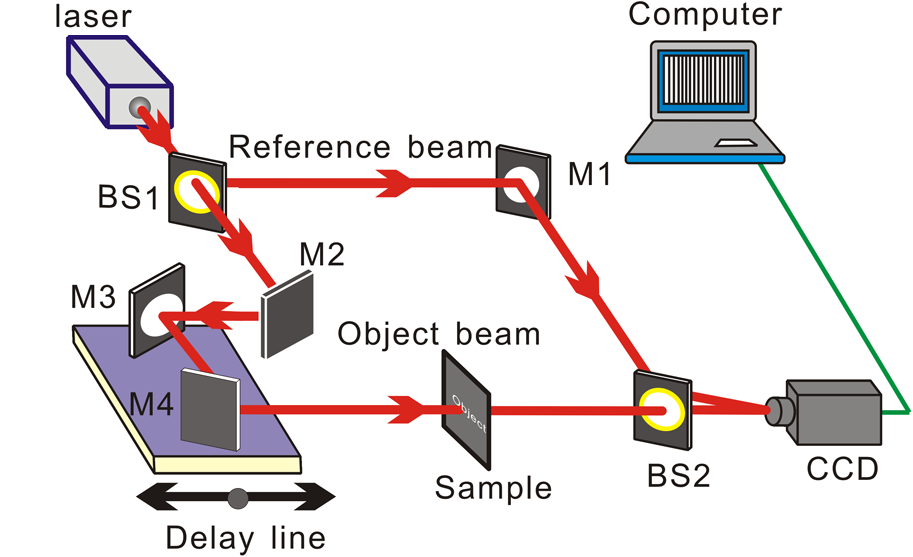
\includegraphics[width=0.8\textwidth]{fig1.png}
  \caption{数字全系成像示意图}
  \label{fig:dh}
\end{figure}

从目标处反射或透射的光到达CCD的过程,可以通过衍射理论来描述。
如图\ref{fig:diffraction}所示,设目标物反射或投射的光场在$\Sigma_0$平面处为$E_0(x_0,y_0)$,
其中$(x_0, y_0)$是$\Sigma_0$平面的坐标,那么利用惠更斯-菲涅尔原理,到达成像平面$\Sigma$的光场为
\begin{equation}
E(x, y; z) = - \frac{i k}{2 \pi z} \iint_{\Sigma_0} dx_0 dy_0 E_0(x_0,y_0) \exp(i k \sqrt{(x-x_0)^2+(y-y_0)^2+z^2})
\label{eq:huygens}
\end{equation}
其中$k=\frac{2 \pi}{\lambda}$为波数,$z$ 是物平面和像平面间的距离。
上式也可以表达为卷积形式
\begin{equation}
E(x,y; z) = E_0(x , y) \ast S_H(x, y; z)
\end{equation}
式中点扩展函数(PSF) $S_H$代表惠更斯球面波,
\begin{equation}
S_H(x, y; z) =  - \frac{i k}{2 \pi z} \exp(i k \sqrt{x^2+y^2+z^2})
\end{equation}
式(\ref{eq:huygens})表示像平面的光场是由物场所有点源发出的球面波的叠加。

\begin{figure}[htb]
  \centering
  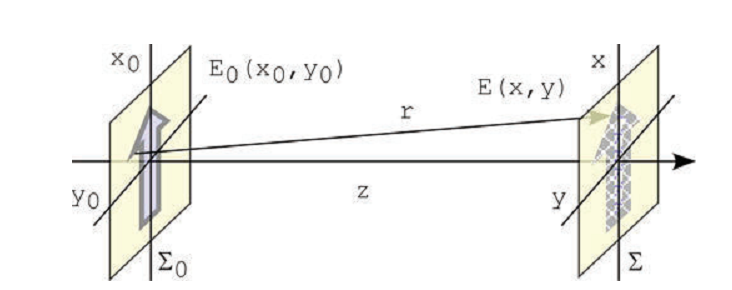
\includegraphics[width=0.8\textwidth]{diffraction.png}
  \caption{衍射过程的示意图}
  \label{fig:diffraction}
\end{figure}

当成像距离满足$z^3\gg\frac{k}{8}[(x-x_0)^2+(y-y_0)^2]_{max}^2$,
则可以利用菲涅尔近似,将点扩展函数改写为
\begin{equation}
S_F(x, y; z) =  - \frac{i k}{2 \pi z} \exp(i k z + \frac{i k}{ 2 z} (x^2+y^2))
\end{equation}
利用菲涅尔近似,可以得到菲涅尔衍射公式
\begin{equation}
\begin{split}
E(x, y; z) &=  \iint_{\Sigma_0}dx_0dy_0 E(x_0,y_0) S_F(x-x_0, y-y_0; z) \\
			&= -\frac{i k}{2 \pi z} e^{i k z} \iint_{\Sigma_0} E(x_0,y_0) e^{ \frac{i k}{ 2 z} [(x-x_0)^2+(y-y_0)^2] } \\
			&= -\frac{i k}{2 \pi z} e^{i k z} e^{\frac{i k }{2 z} (x^2+y^2)} \iint_{\Sigma_0} E(x_0,y_0) e^{ \frac{i k}{ 2 z} (x_0^2+y_0^2)} e^{- \frac{i k}{ z} (x x_0+y y_0)} \\
			&= -\frac{i k}{2 \pi z} e^{i k z} e^{\frac{i k }{2 z} (x^2+y^2)} FT\{E(x_0,y_0) e^{ \frac{i k}{ 2 z} (x_0^2+y_0^2)}\} \vert_{f_x = \frac{x}{\lambda z}, f_y = \frac{y}{\lambda z}}
\end{split}
\label{eq:fresnel}
\end{equation}
其中$FT\{\cdot\}$是傅里叶变换。
从上式来看,菲涅尔衍射的过程可以看做由如下过程合成,
首先物场先经过一个物场二次相因子进行相位畸变,然后经过一个傅里叶变换,
最后再经过像场的二次相因子扭曲。这里略去常数相因子和幅度衰减的影响,并不影响对结果的分析。
因此,要对衍射过程进行数值仿真,只需按照式(\ref{eq:fresnel})做一次傅里叶变换即可,
傅里叶变换可以用快速傅里叶变换(FFT)高效地实现,比如在MATLAB中就有fft2这个函数实现二维的快速傅里叶变换。

设物光为$o(x, y)$,进过衍射到达CCD时为$O(x,y)$,到达CCD的参考光为$R(x,y)$。
CCD最终记录的全息图是二者的干涉图样,即
\begin{equation}
H(x,y) = |O+R|^2 = |O|^2 + |R|^2 +RO^*+R^*O.
\end{equation}
若用原参考光照明CCD记录的全息图,则照明后的光场为
\begin{equation}
\begin{split}
U(x,y) &= R(x,y)H(x,y) \\
		&= R(|O|^2 + |R|^2) + RR^*O + RRO^* \\
		&= T_0 + T_{+1} + T_{-1}
\end{split}		
\end{equation}
式中,$T_0$ 表示与重现光波相同的透射光场,称为零级衍射光;
$T_{+1}$与原始物光波相同,称为+1级衍射光,重现了与原物相同的虚像。
而$T_{-1}$	与原始物光波共轭,称为-1级衍射光,代表共轭实像。

在数字全息成像中,上述重建过程是通过电脑程序数值模拟实现的,
这一过程分为两步,首先用再现光波与CCD探测到的全息图相乘,
然后根据标量衍射理论如菲涅尔衍射公式(\ref{eq:fresnel}),
计算出焦平面的像。在离轴数字全息光路中,三个像是分离的,在后面我将仿真出这个结果。

在平面光照明的离轴数字全息光路中,参考光并不是与CCD垂直的,而是存在一个夹角。
如图\ref{fig:dh}所示,参考光与物光并不平行。
到达CCD的参考光可以表示为
\begin{equation}
R(x,y) = exp[-i k(x \sin \alpha + y \sin \beta)]
\end{equation}
采用菲涅尔近似,根据式(\ref{eq:fresnel}),略去常数相因子和振幅衰减系数,像光可以写为
\begin{equation}
O(x,y) = \iint_{\Sigma_0} o(x_0,y_0) \exp ( \frac{i k}{ 2 z} [(x-x_0)^2+(y-y_0)^2] ) 
\end{equation}
那么,全息图中代表共轭实像的项
\begin{equation}
RO^* = exp[-i k(x \sin \alpha + y \sin \beta)] \iint_{\Sigma_0} o(x_0,y_0) \exp ( -\frac{i k}{ 2 z} [(x-x_0)^2+(y-y_0)^2] ) 
\end{equation}
将与$x$、$y$无关的项合并为$C(x_0,y_0)$,那么上式可以改写为
\begin{equation}
RO^* = \iint_{\Sigma_0} C(x_0,y_0) \exp ( -\frac{i k}{ 2 z} [(x-x_0 + z \sin \alpha)^2+(y-y_0 + z \sin \beta)^2] ) 
\end{equation}
上式可以看做不同的球面波的叠加,也可以看做不同频率的信号的叠加。
其中信号的相位和空间频率分别是
\begin{equation}
P= \frac{k}{ 2 z}[(x-x_0 + z \sin \alpha)^2+(y-y_0 + z \sin \beta)^2] \\
\end{equation}
\begin{equation}
\begin{split}
f_x = \frac{\partial P}{2\pi\partial x} = \frac{x-x_0+z\sin \alpha}{\lambda z} \\
f_y = \frac{\partial P}{2\pi\partial y} = \frac{y-y_0+z\sin \beta}{\lambda z}
\end{split}
\end{equation}

设物体在$x$,$y$方向的线度分别是$X$和$Y$,CCD的尺寸为$L_x, L_y$,
则由物体边缘点$x_0=-X/2, y_0=-Y/2$发出的光,
到达全息图边缘$x=L_x/2, y=L_y/2$时,与参考光的夹角最大,对应的空间频率也最大;
而对应$x_0=X/2,y_0=Y/2$,$x=-Lx/2,y=-L_y/2$
形成的干涉条纹空间频率最小,最大和最小空间
频率分别为
\begin{equation}
\begin{split}
(f_{xmax})_{RO^*} &= \frac{\frac{L_x}{2}+\frac{X}{2}+z\sin\alpha}{\lambda z} \\
(f_{ymax})_{RO^*} &= \frac{\frac{L_y}{2}+\frac{Y}{2}+z\sin\alpha}{\lambda z} \\
(f_{xmin})_{RO^*} &= \frac{-\frac{L_x}{2}-\frac{X}{2}+z\sin\alpha}{\lambda z} \\
(f_{ymin})_{RO^*} &= \frac{-\frac{L_y}{2}+\frac{Y}{2}+z\sin\alpha}{\lambda z}
\end{split}
\label{eq:fmax}
\end{equation}

CCD成像过程需要对干涉图样进行采样,
根据采样定理,采样频率应该是最大空间频率的2倍,
设CCD阵元水平和垂直方向的间隔分别为$\Delta x、\Delta y$,
则有
\begin{equation}
\begin{split}
\frac{\frac{L_x}{2}+\frac{X}{2}+z\sin\alpha}{\lambda z} \le \frac{1}{2\Delta x} \\
\frac{\frac{L_y}{2}+\frac{Y}{2}+z\sin\alpha}{\lambda z} \le \frac{2}{2\Delta y}
\end{split}
\end{equation}

根据上式可以得到参考光的入射角的最大值
\begin{equation}
\begin{split}
\sin\alpha\le\frac{\lambda}{2\Delta x}-\frac{X}{2z}-\frac{L_x}{2z} \\
\sin\beta\le\frac{\lambda}{2\Delta y}-\frac{Y}{2z}-\frac{L_y}{2z}
\end{split}
\label{eq:max_angle}
\end{equation}
这表明由于CCD采样频率的限制,导致入射角的偏置不能太高,
因为空间频率和角度有关,
如果从角谱的角度来理解则很方便,
因为物光与轴的夹角越大,对应的角谱越高,
而参考光的偏置相当于做了频谱搬移,
如果偏置角度太高则会将频谱搬移到空间频率高的地方,
则会让CCD采样出现过大的混叠!

另一方面,偏置角度还受像的可分离性所限制,
之所以采用离轴方式的光路,
就是为了让$T_0、T_{-1}、T_{+1}$三个像在重建的时候能够分离开。
在全息图中,$|R^2|=$常数,频谱是空间频率平面的$\delta$函数,
原始像$R^*O$的频率分布与共轭像$RO^*$共轭,
而$|O|^2=OO*$是物光自相干产生的图样,
它最大空间频率分别为\cite{goodman2006傅里叶光学导论}
\begin{equation}
(f_{xmax})_{|O|^2} =\frac{X}{\lambda z}, 
(f_{ymax})_{|O|^2} =\frac{Y}{\lambda z}
\end{equation}

因此,为了将三个像区分开,要求
\begin{equation}
(f_{xmin})_{RO^*}= (f_xmax)_{|O^2|},
(f_{ymin})_{RO^*}= (f_ymax)_{|O^2|}
\end{equation}
将(\ref{eq:fmax})代入上式可得
\begin{equation}
\begin{split}
\frac{-\frac{L_x}{2}-\frac{X}{2}+z\sin\alpha}{\lambda z} \ge \frac{X}{\lambda z}\\
\frac{-\frac{L_y}{2}+\frac{Y}{2}+z\sin\alpha}{\lambda z} \ge \frac{Y}{\lambda z}
\end{split}
\end{equation}
于是得到离轴菲涅尔全息成像参考光偏置的又一个限制条件,
即再现像分离条件:
\begin{equation}
\begin{split}
\sin \alpha \ge \frac{3X+L_x}{2z} \\
\sin \beta \ge \frac{3Y+L_y}{2z}
\end{split}
\label{eq:min_angle}
\end{equation}

作为一个特例,可以画出当偏置角满足上式最小偏置角时,
$|O|^2$、$RO^*$、$R^*O$的频率分布如图\ref{fig:spectrum}所示。
\begin{figure}[htb]
  \centering
  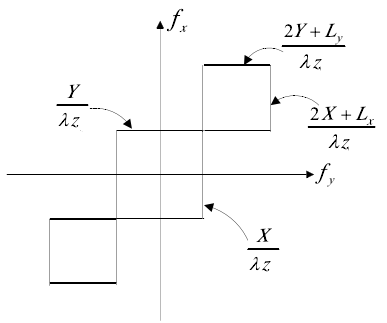
\includegraphics[width=0.5\textwidth]{spectrum.png}
  \caption{临界像可分离情况下3个部分的频谱示意图}
  \label{fig:spectrum}
\end{figure}

根据式(\ref{eq:max_angle},\ref{eq:min_angle}),
可以得到记录距离需要满足的关系
\begin{equation}
z_x\ge\frac{4X+2L_x}{\lambda}\Delta x,
z_y\ge\frac{4Y+2L_y}{\lambda}\Delta y
\end{equation}
因此,离轴菲涅尔全息成像最小记录距离如下
\begin{equation}
z_{min}=max\{\frac{4X+2L_x}{\lambda}\Delta x, \frac{4Y+2L_y}{\lambda}\Delta y\}
\label{eq:min_z}
\end{equation}

只有上式成立,加上满足最小偏置角要求的情况下,
抽样条件才能同时满足,因此式(\ref{eq:min_angle})和
(\ref{eq:min_z})同时构成离轴菲涅尔全息成像的条件。

当全息图的记录条件满足这两个约束之后,
重建的时候用参考光或其共轭与全息图相乘,
然后按照式(\ref{eq:fresnel})计算衍射的像,
在与成像距离相同或相反的地方可以得到再现像。

为了验证此结论,我进行了计算机模拟,并与论文\cite{王华英2008数字全息显微成像的理论和实验研究}
中的结果进行比较。
模拟用的CCD参数为:水平和垂直的像素点为512,
$\Delta x=\Delta y = 0.01mm$,模拟记录的物体大小为1mm$\times$1mm的矩形框,
记录和再现波长均为632.8mm。
与论文\cite{王华英2008数字全息显微成像的理论和实验研究}
比较,可以看出我跟他的结果是非常一致的。
从第3幅子图也可以看出,偏置角的影响,
仿真中选取的偏置角恰好使水平方向可以分离开的临界角,
而在垂直方向则没有偏置。重建时用的不是原始参考光,而是准直光,即相位是常数。

\begin{figure}[htb]
  \centering
  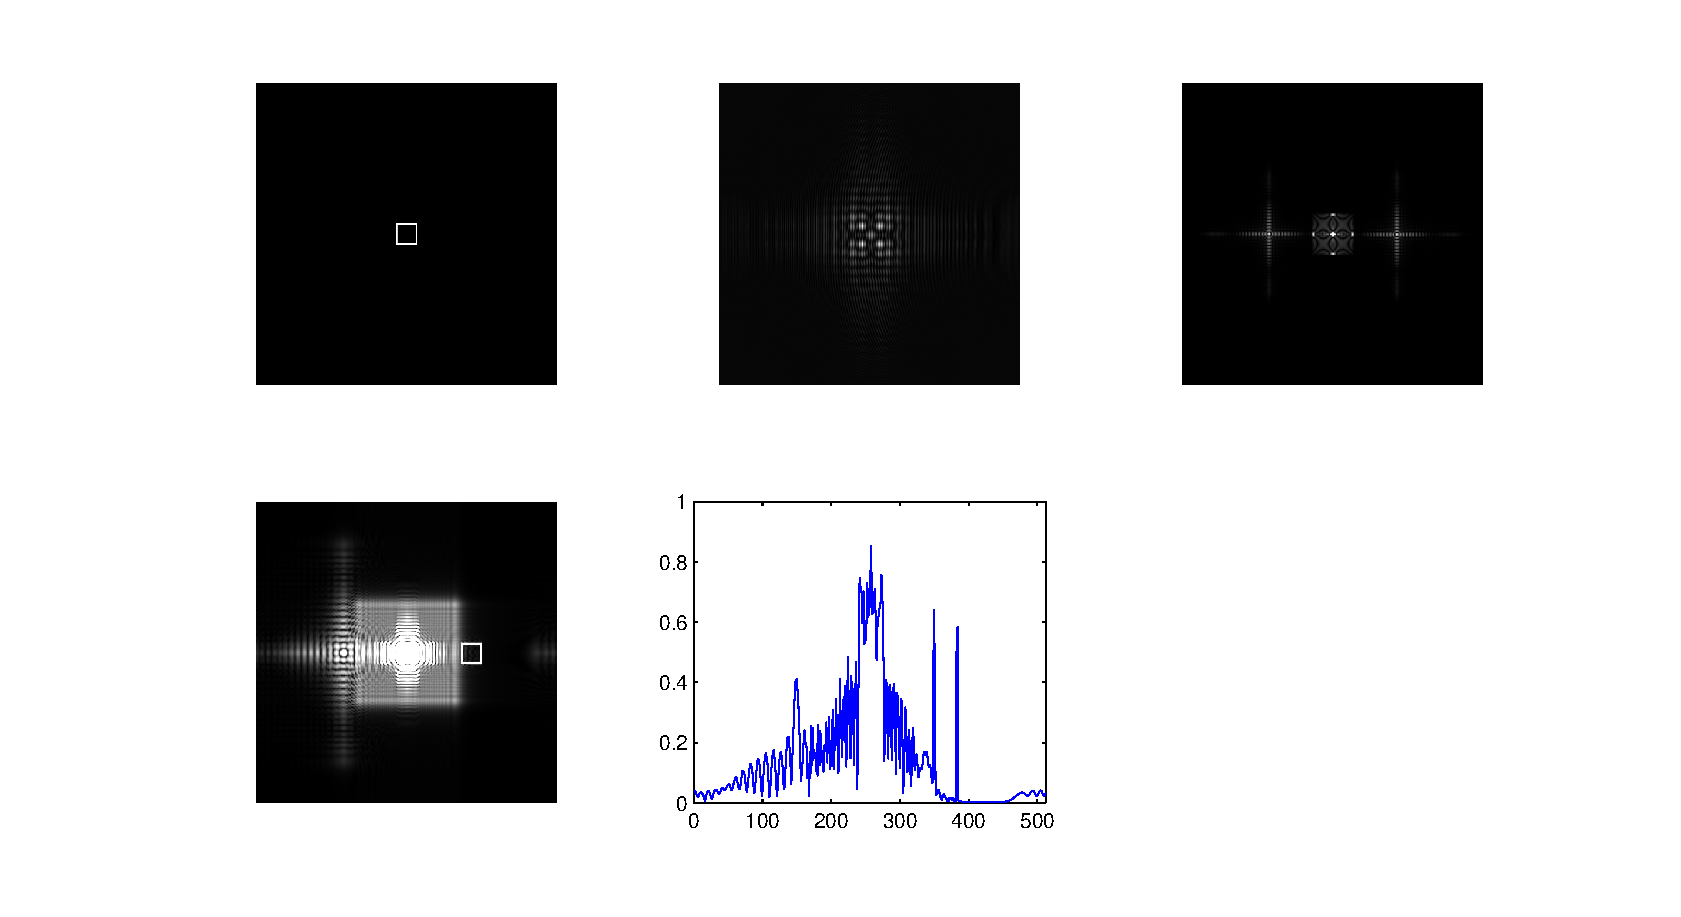
\includegraphics[width=\textwidth]{kuang.eps}
  \caption{菲涅尔数字全息成像仿真结果,依次为,原始目标,全息图,全息图的频谱,菲涅尔重建的强度图,重建强度图的水平中线的强度分布图}
  \label{fig:res_kuang}
\end{figure}

根据重建算法,菲涅尔衍射重建公式,
利用离散傅里叶变换时频域采样间隔的关系,
可以得到这种重建方法的成像分辨率为
\begin{equation}
\Delta x_i = \frac{\lambda z}{N_x \Delta x},
\Delta y_i = \frac{\lambda z}{N_y \Delta y}
\end{equation}

根据仿真的参数设定,计算出成像距离
为最小成像距离225mm,所以成像分辨率为0.028mm。

如果不采用平面参考光照明,而是采用球面光照明,
也可以得到类似的结论,并且用球面波照明还有这样一些好处。
尤其是按照无透镜傅里叶变换全息术的光路时,
干涉条纹接近于平行且等间距,这样可以充分利用CCD的有限带宽。

当采用离轴球面光照明时,到达CCD的参考光在菲涅尔近似下可以写为
\begin{equation}
R(x,y) = exp\{\frac{i k}{2 z_r}[(x-x_r)^2+(y-y_r)^2]\}
\end{equation}
其中$z_r, x_r, y_r$分别是光源离CCD的距离,离轴的水平距离和垂直距离。
和上面进行类似的推导,可以得到偏置$x_r,y_r$以及成像的距离所满足的约束条件
\begin{equation}
\begin{split}
\frac{z_r}{z}\frac{3X}{2} + (\frac{z_r}{z}-1)\frac{L_x}{2} \le x_r \le \frac{\lambda z_r}{2\Delta x} - (\frac{z_r}{z}-1)\frac{L_x}{2}-\frac{z_r}{z}\frac{X}{2} \\
\frac{z_r}{z}\frac{3Y}{2} + (\frac{z_r}{z}-1)\frac{L_y}{2} \le y_r \le \frac{\lambda z_r}{2\Delta y} - (\frac{z_r}{z}-1)\frac{L_y}{2}-\frac{z_r}{z}\frac{Y}{2} 
\end{split}
\end{equation}

对于离轴无透镜傅里叶变换全息成像,记录参考点源位于物平面上,
即$z_r=z$,代入上式,可以得到简化的结果
\begin{equation}
\begin{split}
\frac{3}{2}X\lex_r\le\frac{\lambda z}{2\Delta x} - \frac{X}{2} \\
\frac{3}{2}Y\lex_r\le\frac{\lambda z}{2\Delta y} - \frac{Y}{2} 
\end{split}
\end{equation}
根据上式还可以解出最小成像距离
\begin{equation}
z_{min} = \max(\frac{4X}{\lambda}\Delta x, \frac{4Y}{\lambda} \Delta y )
\end{equation}
\section{总结}


\bibliographystyle{IEEEtran}
\bibliography{ref}

\end{document}